\section{Results from the simulation}

% \subsection{Overview of the interface}

The simulation, as mentioned above, is articulated in three steps, managed by different windows of the GUI. The first is the generation of the speckle fields, 
the second is the spatial filtering together with caculation of the interference patterns using the resulting filtered speckle fileds, the third is the analysis of 
the patterns and the calculation of the correlation function.

% Maybe add some figures here, illustrating the GUI? Or keep that for the notebook?

% \subsection{Generation of the speckle fields} keep this for the notebook?

\subsection{Interference patterns}

The interference patterns produced look like figure \ref{patt}. There are three main effects which in principle have to be taken into account when modeling them: 
the modulation of the cosine (due to the finite width of the slits), the loss of visibility (due to the partial coherence between the field amplitudes at the two slits) and 
an overall reduction of the intensity if compared with coherent light (due to the partial coherence across the two indivudual slits).

\begin{figure}[!ht]
    \centering
    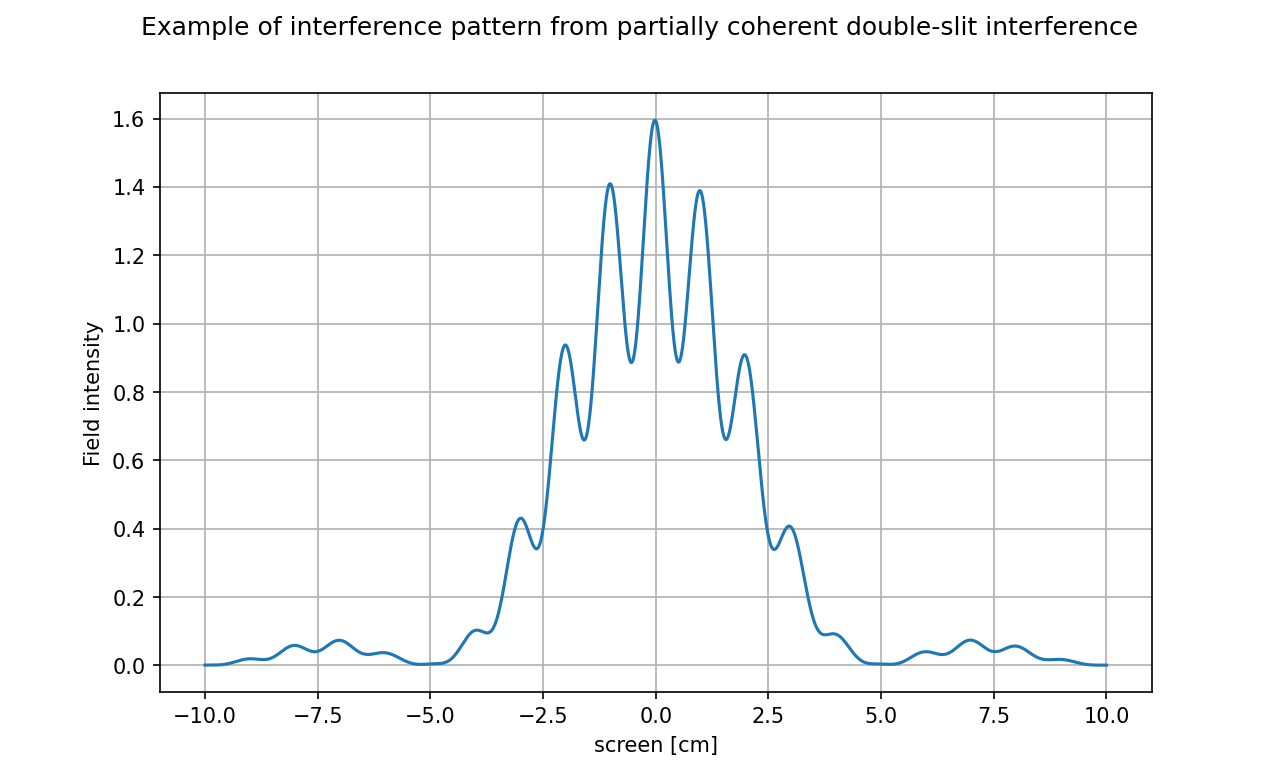
\includegraphics[width = .9\textwidth]{Img/pattern.png}
    \caption{Typical interference pattern}
    \label{patt}
\end{figure}